\documentclass[a4paper,11pt]{article}
\usepackage{fontspec}
\usepackage{color}
\definecolor{citeblue}{rgb}{0.0000,0.4706,0.7216}
\definecolor{titleblue}{rgb}{0.0000,0.4667,0.7137}
\definecolor{titlegreen}{rgb}{0.4078,0.6510,0.3098}
\definecolor{titlecoral}{rgb}{0.8745,0.3922,0.4000}
\definecolor{titleorange}{rgb}{0.9569,0.6353,0.3804}
\definecolor{titleink}{rgb}{0.1608,0.1922,0.2431}
\setmainfont{Times.TTF}[Path=../assets/fonts/,BoldFont=Timesbd.TTF,ItalicFont=Timesi.TTF,BoldItalicFont=Timesbi.TTF]
\usepackage{unicode-math}\setmathfont{texgyretermes-math.otf}
\usepackage{amsmath,siunitx,booktabs,longtable,graphicx,caption,geometry,titlesec,xurl,hyperref,array,fancyhdr}
\geometry{textwidth=5.5in,textheight=9in,centering,headheight=20pt,headsep=10pt}
\makeatletter\renewcommand\normalsize{\@setfontsize\normalsize{11.5}{14}}\makeatother
\AtBeginDocument{\normalsize}
\pagestyle{fancy}\fancyhf{}\fancyhead[L]{EE5110 Technical Report}\fancyhead[R]{A0354063J}\fancyfoot[C]{\thepage}\renewcommand{\headrulewidth}{.3pt}
\titleformat{\section}{\normalfont\fontsize{14}{17}\selectfont}{\thesection}{.7em}{}
\titlespacing*{\section}{0pt}{2ex plus .5ex minus .2ex}{1.5ex plus .3ex minus .2ex}
\titleformat{\subsection}{\normalfont\fontsize{11.5}{14}\selectfont}{\thesubsection}{.7em}{}
\titlespacing*{\subsection}{0pt}{1.8ex plus .5ex minus .2ex}{.8ex plus .2ex}
\DeclareCaptionFont{report}{\fontsize{11.5}{14}\selectfont}\captionsetup{font=report,labelfont=bf,skip=5pt,hypcap=false}
\setlength{\parindent}{0pt}\setlength{\parskip}{6pt}\setlength{\tabcolsep}{4pt}
\setlength{\LTpre}{8pt}\setlength{\LTpost}{8pt}\renewcommand{\arraystretch}{1.06}
\newcolumntype{L}[1]{>{\raggedright\arraybackslash}p{#1}}
\newcolumntype{C}[1]{>{\centering\arraybackslash}m{#1}}
\newcolumntype{R}[1]{>{\raggedleft\arraybackslash}p{#1}}
\hypersetup{colorlinks=true,linkcolor=citeblue,citecolor=citeblue,urlcolor=black,pdftitle={AWISU: Autonomous Warehouse Inventory with a Small UAV},pdfauthor={Junjie Peng}}\urlstyle{same}
\setcounter{topnumber}{2}\setcounter{bottomnumber}{2}\renewcommand{\topfraction}{.90}\renewcommand{\bottomfraction}{.8}\renewcommand{\textfraction}{.10}\renewcommand{\floatpagefraction}{.8}
\emergencystretch=2em\widowpenalty=10000\clubpenalty=10000\displaywidowpenalty=10000
\newcommand{\reportabstracttitle}{A{\fontsize{11.2}{17}\selectfont BSTRACT}}
\setlength{\leftmargini}{3pc}
\renewenvironment{abstract}{\vskip.075in\centerline{\fontsize{14}{17}\selectfont\reportabstracttitle}\vspace{.5ex}\begin{quote}}{\par\end{quote}\vskip1ex}
\AtBeginDocument{\setlength{\abovedisplayskip}{7pt plus2pt minus5pt}\setlength{\belowdisplayskip}{7pt plus2pt minus5pt}\setlength{\abovedisplayshortskip}{0pt plus3pt}\setlength{\belowdisplayshortskip}{4pt plus3pt minus3pt}}
\raggedbottom
\newcommand{\reportneedspace}[1]{\par\begingroup\dimen0=\pagegoal\advance\dimen0 by-\pagetotal\ifdim\dimen0<#1\newpage\fi\endgroup}
\begin{document}
\begin{center}\vspace*{6pt}{\fontsize{17.28}{20}\selectfont \textcolor{titleblue}{A}\textcolor{titlegreen}{W}\textcolor{titlecoral}{I}\textcolor{titleorange}{S}\textcolor{titleblue}{U}: \textcolor{titleblue}{A}{\fontsize{13.82}{14}\selectfont UTONOMOUS} \textcolor{titlegreen}{W}{\fontsize{13.82}{14}\selectfont AREHOUSE}\\\textcolor{titlecoral}{I}{\fontsize{13.82}{14}\selectfont NVENTORY} {\fontsize{13.82}{14}\selectfont WITH} {\fontsize{13.82}{14}\selectfont A} \textcolor{titleorange}{S}{\fontsize{13.82}{14}\selectfont MALL} \textcolor{titleblue}{U}AV\par}\vspace{12pt}\textbf{Junjie Peng}\\[8pt]\href{https://github.com/JackyPengJJ/AWISU}{\raisebox{-2pt}{
\includegraphics[height=11.5pt]{figures/github.pdf}} Code}\quad\href{https://youtu.be/ZQHlchVMqs8}{\raisebox{-2pt}{
\includegraphics[height=10pt]{figures/youtube.pdf}} YouTube}\end{center}
\begin{abstract}
We present AWISU, a small-UAV design for bilateral barcode inventory in an unknown, GPS-denied warehouse aisle. The design combines LiDAR-inertial-visual navigation, two pitch-adjustable global-shutter cameras, a spatial inventory record and immediate local recovery. Complete-label projection constrains continuous scanning to 0.85 m/s for the supported label geometry. Installed mass is 2901.6 g including 100 g contingency; individual flight and recovery actions determine mission duration and energy. A 400-item scenario with two recoveries takes 669.5 s and requires 73.63 Wh under adverse power assumptions, or 92.04 Wh delivered while retaining a 20\% reserve. MuJoCo studies evaluate tracking, decoding and matched-design execution. The selected residual controller reduces full-route RMSE from 0.1148 to 0.1038 m; crop verification recovers 400 item IDs from 1420 images. Matched execution reaches 0.0138 m RMSE at 25.84 A peak model current.

\end{abstract}
\section{I{\fontsize{11.2}{14}\selectfont NTRODUCTION}}
Warehouse inventory requires both readable barcodes and spatial coverage. Each observation must identify a physical cargo instance; empty, unseen and unresolved locations need distinct records. A clearer image may require a closer viewpoint, consuming energy needed to finish the aisle.

The assignment specifies an 80×2.5×8 m aisle, five equally spaced cargo levels on each side, aisle-facing barcodes, mass below 3 kg and one-flight completion. Rack poses, obstacles and cargo locations are unknown. These constraints couple platform choice, autonomous control and GPS-free navigation.

AWISU combines bilateral pitch heads, a continuous five-level snake and immediate local recovery. Figure~\ref{fig:1} connects complete-label visibility, motion admission and an action-based energy budget. The worked scenario retains 400 cargo units and the reference scene’s 100×44 mm short-code labels; neither quantity nor label size is prescribed by the assignment. The aisle is static and access-controlled. Label density, connection loss and recovery workload are varied; battery calculations use 23 °C source curves.

\par\addvspace{2pt}\noindent\begin{minipage}{\linewidth}\centering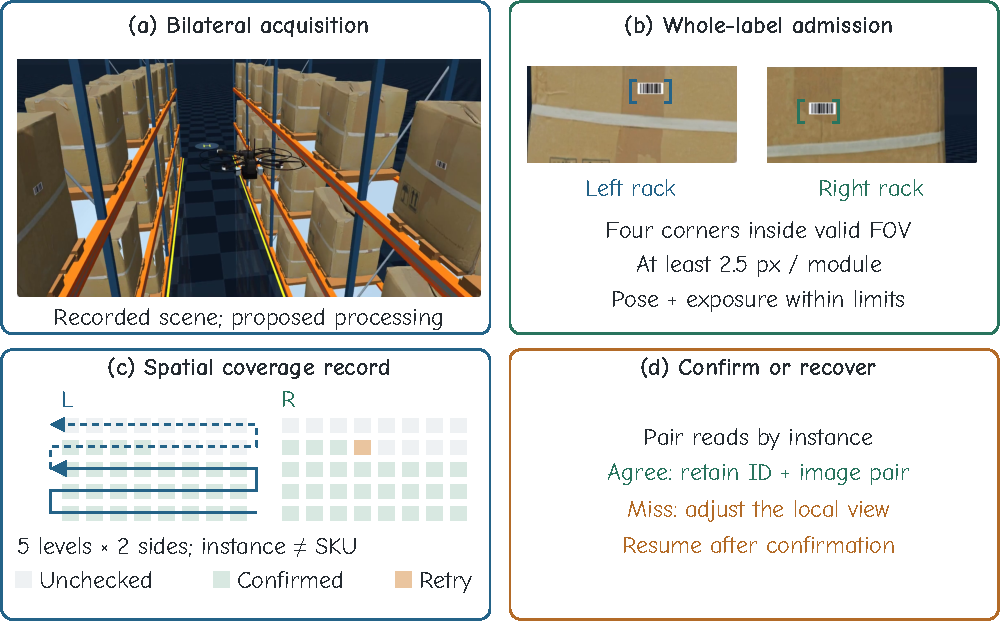
\includegraphics[width=\textwidth]{figures/framework.pdf}
\captionof{figure}{AWISU overview. Recorded images show acquisition; coverage states and recovery illustrate the proposed task logic. Solid and dashed paths denote covered and planned travel.}\label{fig:1}\end{minipage}\par\addvspace{2pt}
\section{R{\fontsize{11.2}{14}\selectfont ELATED} W{\fontsize{11.2}{14}\selectfont ORK} {\fontsize{11.2}{14}\selectfont AND} D{\fontsize{11.2}{14}\selectfont ESIGN} C{\fontsize{11.2}{14}\selectfont HOICES}}
\subsection{I{\fontsize{9.2}{14}\selectfont NVENTORY} {\fontsize{9.2}{14}\selectfont WORKFLOW} {\fontsize{9.2}{14}\selectfont AND} {\fontsize{9.2}{14}\selectfont AIRCRAFT} {\fontsize{9.2}{14}\selectfont PLATFORM}}
Corvus One \cite{r3} and Verity \cite{r4} organise inventory around repeated observations, location association and warehouse records. AWISU adopts this organisation: each confirmed item retains image evidence and a spatial identity, while failed reads enter a recovery queue. Component specifications and mission calculations determine aircraft sizing.

Platform alternatives include a documented development kit, a custom quadrotor and a hexarotor. Holybro's X500 v2 uses a 500 mm frame, 2216 KV920 motors, 4S ESCs and 1045 propellers \cite{r5}. We select a 600 mm custom frame to accommodate protected 14-inch rotors. Its larger disc area reduces loading, at the expense of aisle clearance and custom structure. A hexarotor adds actuators and protection area within the same mass limit.

\par\addvspace{8pt}\noindent\begin{minipage}{\linewidth}\centering
\captionof{table}{Platform alternatives for the warehouse task.}\label{tab:1}
\begin{tabular}{C{0.290\dimexpr\linewidth-24pt\relax}C{0.290\dimexpr\linewidth-24pt\relax}C{0.420\dimexpr\linewidth-24pt\relax}}
\toprule
\textbf{Platform} & \textbf{Useful capability} & \textbf{Limiting trade-off}\\\midrule
Commercial \cite{r3,r4} & Integrated inventory workflow & Component detail unavailable\\
X500 v2 \cite{r5} & Documented PX4 kit & Stock 4S / 10-inch propulsion\\
Custom quadrotor & 600 mm; 14-inch rotors & Custom structure; selected\\
Hexarotor & More actuators & Added mass and guarded area\\
\bottomrule\end{tabular}\end{minipage}\par\addvspace{8pt}
\subsection{N{\fontsize{9.2}{14}\selectfont AVIGATION} {\fontsize{9.2}{14}\selectfont IN} {\fontsize{9.2}{14}\selectfont REPETITIVE} {\fontsize{9.2}{14}\selectfont AISLES}}
Repeated uprights weaken along-aisle observability; plain cartons weaken image tracking. ORB-SLAM3 uses images/IMU \cite{r20}, FAST-LIO2 uses LiDAR/IMU \cite{r19}, and FAST-LIVO2 fuses geometric and photometric residuals \cite{r21}. The latter is selected for complementary cues, accepting calibration/timing work. FAST-LIO2 supplies a geometry-only fallback.

\par\addvspace{8pt}\noindent\begin{minipage}{\linewidth}\centering
\captionof{table}{Navigation alternatives and warehouse trade-offs.}\label{tab:2}
\begin{tabular}{C{0.290\dimexpr\linewidth-24pt\relax}C{0.290\dimexpr\linewidth-24pt\relax}C{0.420\dimexpr\linewidth-24pt\relax}}
\toprule
\textbf{Method} & \textbf{Measurements} & \textbf{Warehouse trade-off}\\\midrule
ORB-SLAM3 \cite{r20} & Images + IMU & Low mass; texture dependence\\
FAST-LIO2 \cite{r19} & LiDAR + IMU & Geometry; axial degeneracy\\
FAST-LIVO2 \cite{r21} & LiDAR + images + IMU & Complementary cues; calibration\\
\bottomrule\end{tabular}\end{minipage}\par\addvspace{8pt}
\subsection{C{\fontsize{9.2}{14}\selectfont ONTROL} {\fontsize{9.2}{14}\selectfont AND} {\fontsize{9.2}{14}\selectfont SAFE} {\fontsize{9.2}{14}\selectfont TRAJECTORY} {\fontsize{9.2}{14}\selectfont EXECUTION}}
PX4’s cascaded position/velocity and attitude/rate loops are selected for firmware support and low computation \cite{r42}, with explicit tilt, thrust and shared-current limits. Table 3 compares geometric feedback \cite{r40}, LQR \cite{r45} and MPC \cite{r41}. A bounded learned residual is evaluated separately \cite{r28,r29}.

\par\addvspace{8pt}\noindent\begin{minipage}{\linewidth}\centering
\captionof{table}{Controller comparison for narrow-aisle flight.}\label{tab:3}
\begin{tabular}{C{0.290\dimexpr\linewidth-24pt\relax}C{0.290\dimexpr\linewidth-24pt\relax}C{0.420\dimexpr\linewidth-24pt\relax}}
\toprule
\textbf{Controller} & \textbf{Constraint handling} & \textbf{Selection trade-off}\\\midrule
Cascaded PID \cite{r42} & Saturation / anti-windup & PX4 implementation; selected\\
Geometric \cite{r40} & Added actuator constraints & Nonlinear attitude; inertia model\\
LQR \cite{r45} & Added saturation checks & Local model; low compute\\
MPC \cite{r41} & Predicted state/input limits & Solver deadline; model sensitivity\\
\bottomrule\end{tabular}\end{minipage}\par\addvspace{8pt}
Planning adopts FASTER’s observed-free stopping backup \cite{r22}. Short local segments and inventory frontiers fit the optical speed limit; a late update leaves the accepted stopping trajectory executable.

\section{S{\fontsize{11.2}{14}\selectfont YSTEM} D{\fontsize{11.2}{14}\selectfont ESIGN} {\fontsize{11.2}{14}\selectfont AND} M{\fontsize{11.2}{14}\selectfont ETHOD}}
\subsection{H{\fontsize{9.2}{14}\selectfont ARDWARE} {\fontsize{9.2}{14}\selectfont AND} {\fontsize{9.2}{14}\selectfont INSTALLATION}}
We select four T-MOTOR MN3508 KV380 motors, P14×4.8 carbon propellers and AIR40A 2–6S ESCs \cite{r6,r7,r8}. GEPRC specifies its 6S2P VTC6 pack at 6000 mAh, 607 g and 30 A continuous discharge \cite{r37}; we allocate 627 g installed. A plastic-case Pixhawk 6C and analog PM02 V3 provide flight control and voltage/current monitoring \cite{r10,r11}. MID-360 supplies LiDAR/IMU observations, OAK-D Lite supplies forward stereo and navigation images, and an Orin Nano 8 GB module runs on a Hiwonder Mini carrier \cite{r12,r13,r14,r15}. The 180 g computer allocation includes the 77 g carrier, module, cooling, storage and supports.

Each side head uses a BFS-U3-122S6M-C: 4096×3000 pixels, 3.45 μm pitch, global shutter, 36 g and 3 W maximum \cite{r35}. A 12 mm RT-V1228-MPY2 lens covers the 1.1-inch sensor \cite{r36}. Its 110 g installed allocation covers the 97 g catalogue lens, mounting and variation. Two pitch assemblies receive 70 g for servos, balance and supports \cite{r18}. Figure~\ref{fig:2} links a reference mesh to these component roles; opposing cameras observe both racks during translation.

\par\addvspace{2pt}\noindent\begin{minipage}{\linewidth}\centering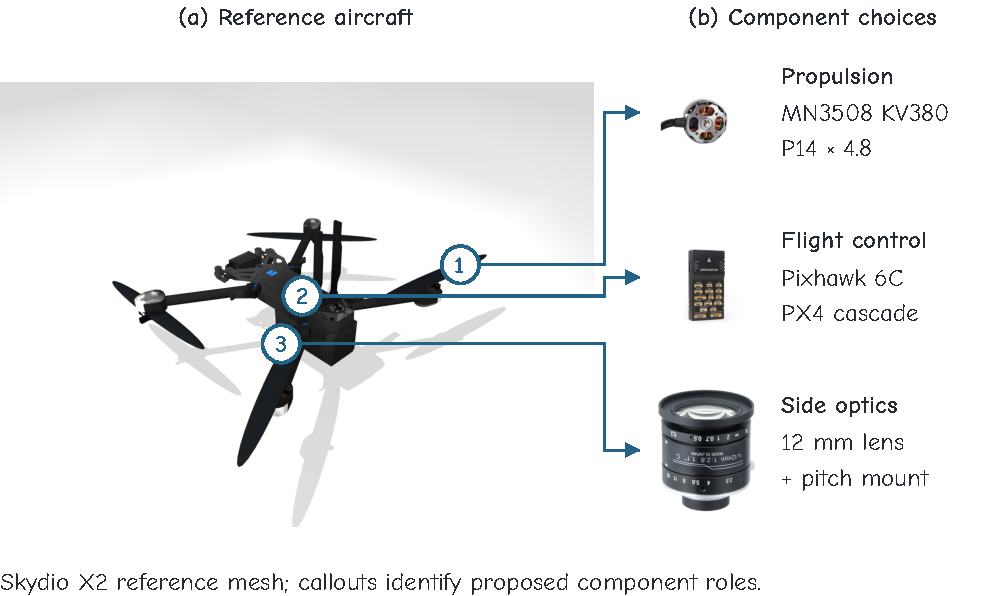
\includegraphics[width=\textwidth]{figures/hardware.pdf}
\captionof{figure}{Reference aircraft and selected components. Render: Skydio X2 \cite{r30}; product photos: T-MOTOR \cite{r6}, Holybro \cite{r10}, Opto Engineering \cite{r36}. Callouts identify proposed component roles.}\label{fig:2}\end{minipage}\par\addvspace{2pt}
We reject the 5 MP/8 mm option because its 55 g lenses reduce mass but require approximately 1.61 mm barcode modules under the baseline uncertainty envelope \cite{r16,r17}. Our 12.3 MP installation adds 130 g in lenses/supports for improved sampling. With these optics, the 755 g 5 Ah LiPo exceeds the mass limit \cite{r9}. Flywoo's 596.2 g P30B pack saves 10.8 g, but its published 35 A description leaves continuous pack current unspecified \cite{r39}. We accept the GEPRC mass penalty for its documented continuous rating. Amprius's 465 g option supplies 12 A continuous, below the approximately 20 A low-voltage mission demand \cite{r44}. A same-mass 20 MP BFS-U3-200S6 offers 2.4 μm pixels but uses rolling shutter with global reset \cite{r46}; it requires a different exposure model. The global-shutter head is retained for the analysed moving acquisition.

\reportneedspace{8\baselineskip}\begin{longtable}{C{0.440\dimexpr\linewidth-24pt\relax}C{0.130\dimexpr\linewidth-24pt\relax}C{0.430\dimexpr\linewidth-24pt\relax}}
\caption{Installed mass budget.}\label{tab:4}\\
\toprule
\textbf{Item} & \textbf{Mass (g)} & \textbf{Basis}\\\midrule
\endfirsthead
\toprule
\textbf{Item} & \textbf{Mass (g)} & \textbf{Basis}\\\midrule
\endhead
Frame / landing supports & 340 & Geometry allocation\\
4 x MN3508 KV380 & 412 & Manufacturer \cite{r6}\\
4 x AIR40A ESC & 104 & Installation allocation \cite{r7}\\
4 x P14x4.8 & 66 & Manufacturer \cite{r8}\\
Propeller rings and bracing & 140 & Custom-part allocation\\
Pixhawk 6C (plastic) & 34.6 & Manufacturer \cite{r10}\\
PM02 V3 analog module & 20 & Manufacturer \cite{r11}\\
MID-360 & 265 & Manufacturer \cite{r12}\\
OAK-D Lite fixed-focus & 61 & Product installation reference \cite{r13}\\
Orin Nano assembly & 180 & Module / carrier / cooling \cite{r14,r15}\\
2 x BFS-U3-122S6M-C & 72 & Manufacturer \cite{r35}\\
2 x RT-V1228-MPY2 & 220 & 110 g each installed \cite{r36}\\
Paired pitch supports & 70 & 70 g installed \cite{r18}\\
VTC6 6S2P 6 Ah & 627 & 607 g + 20 g installed \cite{r37}\\
Regulators / LEDs / harness & 150 & Installation allocation \cite{r11,r33,r34}\\
Sensor mounts and isolators & 40 & Custom-part allocation\\
Integration contingency & 100 & Explicit design allowance\\
\textbf{Total installed} & \textbf{2901.6} & \textbf{Includes 100 g contingency}\\
\bottomrule\end{longtable}
The 2901.6 g total includes 100 g contingency and leaves 98.4 g to the limit. Custom structure uses two 180×140×2 mm carbon plates and four 16/14 mm outer/inner-diameter tubes, approximately 240 mm long. At 1600 kg/m³ these contribute 161 g and 72 g; the remainder of the 340 g frame allocation covers joints, fasteners and landing supports. Rings/bracing receive a separate 140 g. Substitutions must fit installed allocations, including cables and supports.

Adjacent motors are $0.600/\sqrt{2}=0.424$ m apart. With 0.3556 m rotors and two 0.020 m radial protection allowances, protected discs remain 0.029 m apart. Rounding the 0.996 m enclosing diameter gives a 1.00 m collision envelope of 0.50 m height. Side optical centres lie at $y=\pm0.40$ m, level with the body reference, with principal rays outside the rotors. Battery placement below the plates balances the elevated LiDAR and outboard optics.

Bank changes the swept envelope. For radius $r=0.50$ m and half-height $h=0.25$ m, lateral extent is $r\cos\theta+h\sin\theta$. At 12°, subtracting that extent and tracking/localisation/map allowances of 0.15/0.15/0.05 m from the 1.25 m half-aisle leaves 0.359 m. At the 7.2 m upper scan height, vertical extent is $r\sin\theta+h\cos\theta$; allowances of 0.10/0.075/0.025 m leave 0.252 m ceiling clearance. Scan admission requires lateral sigma ≤0.05 m and vertical sigma ≤0.025 m; rack protrusions are checked against the same tilted envelope.

\subsection{P{\fontsize{9.2}{14}\selectfont OWER}, {\fontsize{9.2}{14}\selectfont INTERFACES} {\fontsize{9.2}{14}\selectfont AND} {\fontsize{9.2}{14}\selectfont COMPUTATION}}
A fused 6S branch feeds the ESCs; PM02 V3 powers Pixhawk separately. D36V50F12 regulates the computer, LiDAR and LEDs to 12 V; D36V50F6 supplies an isolated 6 V servo rail \cite{r11,r33,r34}. Regulation keeps the carrier below its 19 V maximum at 25.2 V full pack charge. The electrical operating range is 18.0–25.2 V. The 60 W auxiliary allocation covers computing, sensors, lighting and regulators; converter thermal/current curves determine continuous branch admission.

MID-360 connects through Livox driver2 over Ethernet, preserving per-point acquisition offsets for deskewing. OAK-D Lite supplies calibrated stereo/depth and grayscale images over USB. We specify an adapter for the image model, intrinsics, exposure timestamps and extrinsics required by FAST-LIVO2 \cite{r21,r43}. Integration measures clock offset/drift against a 1 ms alignment target. At 1 m/s that offset contributes 1 mm translation; a 0.2° camera–LiDAR rotation error contributes about 17 mm at 5 m, so rotational calibration dominates this example.

The estimator interface registers its body frame to Pixhawk FRD and converts local output to NED for MAVLink ODOMETRY, including covariance, resets and acquisition timestamps \cite{r23}. PX4 receives smooth local odometry and 50 Hz setpoints over 921600-baud UART. A 250-byte odometry message at 50 Hz uses 12.5 kB/s; our 20 kB/s control/telemetry allocation fits approximately 92 kB/s before framing overhead. Stabilisation and the stopping backup run onboard independently of inventory and ground-link queues \cite{r24}.

\par\addvspace{8pt}\noindent\begin{minipage}{\linewidth}\centering
\captionof{table}{Input scale and bounded resource allocations.}\label{tab:5}
\begin{tabular}{C{0.290\dimexpr\linewidth-24pt\relax}C{0.290\dimexpr\linewidth-24pt\relax}C{0.420\dimexpr\linewidth-24pt\relax}}
\toprule
\textbf{Function} & \textbf{Input / allocation} & \textbf{Deadline or overload action}\\\midrule
Estimation & 200 Hz IMU; 10 Hz LiDAR; 30 Hz images & 50 Hz output; stop scan after 0.15 s correction age\\
Map / planner & 10 Hz map; 5 Hz plan; 0.10 m grid & Retain known-free stopping backup\\
Side images & Two 4096×3000 Mono8; 10 fps each & 245.76 MB/s; decode native crops\\
Image queues & Two frames per camera; 49.15 MB & Bound queues; pause missed admission\\
Occupancy & 30×5×10 m; 0.10 m cells & 24 MB cells; 256 MB with indices/history\\
Application & 512 MB map; 128 MB buffers & 3.5 GB application; about 2 GB OS\\
\bottomrule\end{tabular}\end{minipage}\par\addvspace{8pt}
LiDAR adds 4.8 MB/s (200k points/s, 24 bytes/point); 640×400 stereo adds 15.36 MB/s at 30 Hz, totalling about 266 MB/s. Pair bursts reach 20 fps/side. Staggered transfers, bounded queues and native-crop decoding limit load. Four-frame bursts contain 49.15 MB. At a required 400 MB/s usable USB payload rate, reserving 15.36 MB/s for stereo clears the burst in 128 ms; the second pair arrives 50 ms later, leaving 22 ms of its 100 ms deadline for crop processing. These are admission targets for the 15 W mode; overload pauses coverage. A 64 GB drive stores records and selected evidence.

\subsection{D{\fontsize{9.2}{14}\selectfont YNAMICS} {\fontsize{9.2}{14}\selectfont AND} {\fontsize{9.2}{14}\selectfont FLIGHT} {\fontsize{9.2}{14}\selectfont CONTROL}}
We model position $\boldsymbol p$, velocity $\boldsymbol v$, body-to-world attitude $R$, body rate $\boldsymbol\omega$, total thrust $f$ and moment $\boldsymbol\tau$ in an upward-positive local frame \cite{r40}:
\begin{equation}\begin{aligned}\dot{\boldsymbol p}&=\boldsymbol v,\quad m\dot{\boldsymbol v}=Rf\boldsymbol e_3-mg\boldsymbol e_3+\boldsymbol d_f,\\ \dot R&=R[\boldsymbol\omega]_\times,\quad J\dot{\boldsymbol\omega}=\boldsymbol\tau-\boldsymbol\omega\times J\boldsymbol\omega+\boldsymbol d_\tau.\end{aligned}\end{equation}
The controller interface converts this convention to NED/FRD. Rotor thrust and reaction torque follow $f_i=k_T\Omega_i^2$ and $q_i=k_Q\Omega_i^2$, with first-order motor lag. Our reference simulation uses 40 ms lag and 200 Hz integration. The deployment cascade tracks position, velocity and acceleration, then computes orientation and allocates moments through PX4's attitude/rate loops \cite{r42}.

Position/velocity feedback generates a desired acceleration, with clamped integral correction. Reference horizontal gains 2.5 $\mathrm{s}^{-2}$/2.6 $\mathrm{s}^{-1}$ give a 1.58 rad/s natural frequency and 0.82 damping ratio; vertical gains 4.0/3.2 give 2.0 rad/s and 0.80. A 2 Hz attitude target separates the inner and outer loops. Saturation and invalid estimates freeze integration; loaded response measurements determine deployment gains.

Motor/ESC/propeller groups contribute approximately 0.026 kg m² roll/pitch inertia at 0.212 m offsets. A component placement ledger and the parallel-axis theorem give $J_{xx}=0.1026$, $J_{yy}=0.0534$ and $J_{zz}=0.1330$ kg m². Lateral cameras increase roll/yaw inertia substantially. The full matrix, including products of inertia, defines the matched validation plant. The ledger records estimated installation masses and positions. Current-aware allocation takes the form of weighted wrench fitting:
\begin{equation}\boldsymbol f^\star=\arg\min_{0\le f_i\le f_{max}(V)}\|W(B\boldsymbol f-\boldsymbol w_c)\|_2^2\quad\mathrm{s.t.}\quad\sum_i P_i(f_i,V)+P_{aux}\le VI_{max}.\end{equation}
Here $B$ maps thrusts to wrench, $\boldsymbol w_c$ is the demand, and $W$ prioritises collective and roll/pitch before yaw. The matched test implements this priority with bounded scaling and checks every command against the 30 A shared limit. Its power model uses the measured 22.2 V map with explicit installation and low-voltage screening factors; the retained reference run uses inverse allocation with per-rotor clipping. At 0.85 m/s, 0.10 s latency and 0.6 m/s² braking imply 0.687 m stopping distance. A 1.5 m observed corridor includes mapping/tracking margins; a shorter corridor reduces admissible speed.

\subsection{S{\fontsize{9.2}{14}\selectfont TATE} {\fontsize{9.2}{14}\selectfont ESTIMATION} {\fontsize{9.2}{14}\selectfont AND} {\fontsize{9.2}{14}\selectfont LOCAL} {\fontsize{9.2}{14}\selectfont GEOMETRY}}
FAST-LIVO2 propagates position, velocity, attitude and inertial biases, then applies timestamped LiDAR/image corrections \cite{r21,r43}. PX4 retains inertial stabilisation. Exposure, clock, distortion and extrinsic calibration share one transformation chain. Information conditioning, correspondence count, innovations and visual consistency jointly detect repetitive-bay ambiguity. Weak along-aisle information requests a rack-end or cross-bracing view. Map corrections update a map-to-odometry transform, preserving control-frame continuity.

Our local voxel map distinguishes occupied, observed-free and unknown space, following OctoMap \cite{r25}. Planning uses a 0.10 m grid with underlying-point queries near obstacles; pruning preserves the return corridor and rack locations. Initialisation aligns gravity, defines an origin and fits floor/parallel rack planes. Upright clusters define bays; support and cargo surfaces define the task's five height bands. Observed surfaces define scan regions.

Initial geometry thresholds are RANSAC residual ≤max(0.03 m, 3σ\_range), five consistent 10 Hz plane updates, <5° normal disagreement and 0.10 m upright/height clustering. These are initial tuning settings. Ambiguous bands pause association and request another view. Endpoint confirmation requires observed rack termination and a free inflated turn volume. Spatial association combines a 3σ gate, projected face overlap and side/band identity; ambiguous matches remain tentative. Empty slots require observed free faces.

MID-360's −7° to +52° elevation range leaves a lower blind region \cite{r12}. We mount forward stereo approximately 15° downward and yaw 180° at each endpoint so it faces the next pass. Four inter-level turns plus a fifth before return cost 20 s. Keeping heading would save this time but require rear sensing or stricter LiDAR-only admission. Climb/descent requires recently observed free columns and ceiling clearance at the highest band. Figure~\ref{fig:3} quantifies clearance and nominal ray limits; installed geometry supplies additional body/rotor occlusion checks.

\par\addvspace{2pt}\noindent\begin{minipage}{\linewidth}\centering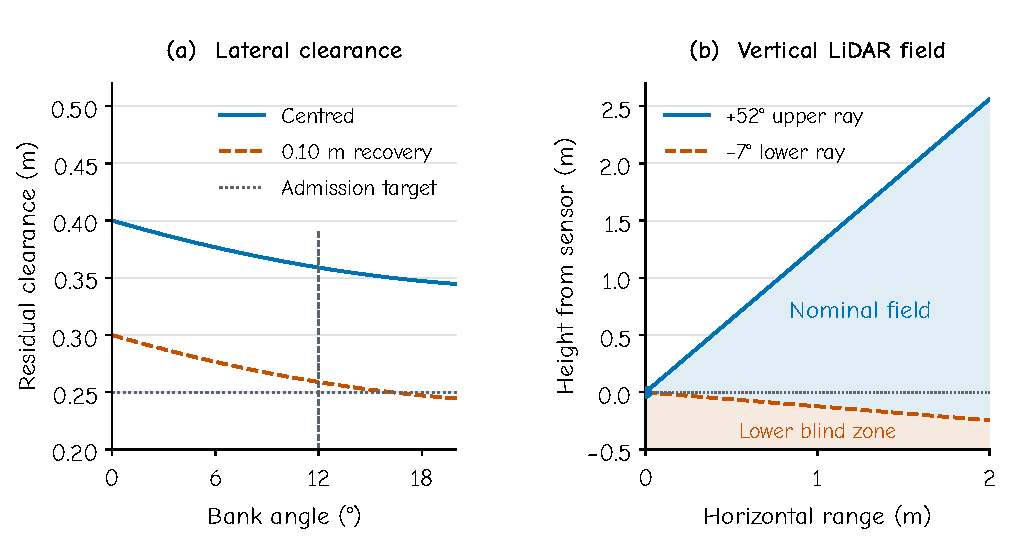
\includegraphics[width=\textwidth]{figures/04_observability.pdf}
\captionof{figure}{Motion limits and sensing envelope. Clearance includes tracking, localisation and map margins; the lower blind zone requires a previously mapped descent column.}\label{fig:3}\end{minipage}\par\addvspace{2pt}
\subsection{C{\fontsize{9.2}{14}\selectfont OVERAGE}, {\fontsize{9.2}{14}\selectfont CONFIRMATION} {\fontsize{9.2}{14}\selectfont AND} {\fontsize{9.2}{14}\selectfont LOCAL} {\fontsize{9.2}{14}\selectfont RECOVERY}}
At 5 Hz, the local planner receives state/covariance, the map, coverage records and remaining energy. It inflates obstacles by the tilted envelope, finds a short path and fits a timed segment with a stopping backup \cite{r22}. Collision, speed, acceleration and reserve checks precede replacement of the current plan. A late update leaves the accepted backup executable. A blocked endpoint selects another mapped transition column; otherwise we return with a blocked-region record.

Each cargo record uses side, bay/band and spatial track as its key, with payload, observation times, covariance and confirmation state as attributes. This preserves distinct instances of repeated SKUs. An action is admitted when:
\begin{equation}\mathcal A(a)=\mathcal L\land\mathcal F(a)\land\mathcal O(a)\land\left[E_{rem}\ge E_a+E_{unfinished}+E_{return}+0.20E_{del}\right].\end{equation}
$\mathcal L$ checks current localisation; $\mathcal F$ checks the swept volume and backup; $\mathcal O$ checks image eligibility whenever a surface is marked inspected. Remaining workload $E_{unfinished}$ updates when cargo or blocked space is discovered. A surface becomes complete after eligible image evidence covers its inspected boundary.

Initialisation supplies the origin and verified stopping corridor. Local geometry then extends the rack frontier; image/pose gates update spatial cargo tracks. Failed tracks enter immediate recovery, endpoint/free-column checks release the next height band, and coverage plus reserve determines completion or return with exceptions.

Each side carries two off-axis LUXEON Rebel LXML-PWC1-0100 LEDs in a 0.70 A series string driven by TPS92512 from 12 V \cite{r34}. A 30° beam covers about 0.16 m² at 0.85 m; 360 lm gives approximately 2 klx before losses, motivating a 0.20 ms exposure. The decoder detects candidates at reduced resolution, reads native crops with zxing-cpp \cite{r26}, checks payload syntax and associates each crop using its exposure pose and calibrated pitch.

Confirmation requires consistent, quality-checked whole-label reads from two acquisitions of the same spatial track. Disagreement triggers a changed exposure or viewpoint. An unreadable carton remains an unresolved instance; confirmed aisle-visible units are counted per SKU and any encoded quantity is parsed separately. Empty, unseen, inaccessible and undecodable locations retain different states.

A failed read preserves opposite-side confirmations and freezes the unfinished boundary. Recovery starts with an in-view retry, followed by braking, recentering and an optional approach up to 0.10 m towards the failed side. Aimed pitch/height replaces the normal sweep during this settled read. With 0.70–0.85 m range and the adopted errors, the centred zero-pitch view retains a 0.619 m safe label-centre interval. A 0.10 m offset leaves 0.259 m lateral clearance against the 0.25 m target and improves centre-ray sampling by about 13\%. Smaller free space or larger uncertainty reduces the offset. Both outward and return sweeps must pass collision checks before scanning resumes at the same boundary.

Each failed item receives at most two settled attempts. Completion requires both sides and all five bands inspected, every observed instance confirmed and no unchecked reachable surface boundary. Persistent failures produce an inventory with exceptions; reserve admission selects return when further recovery cannot be afforded.

\section{D{\fontsize{11.2}{14}\selectfont ESIGN} A{\fontsize{11.2}{14}\selectfont NALYSIS}}
\subsection{C{\fontsize{9.2}{14}\selectfont OMPLETE}-{\fontsize{9.2}{14}\selectfont LABEL} {\fontsize{9.2}{14}\selectfont VISIBILITY} {\fontsize{9.2}{14}\selectfont AND} {\fontsize{9.2}{14}\selectfont ACQUISITION}}
The selected optics give $f_x=12/0.00345=3478$ pixels and approximately 61.0° horizontal/46.7° vertical field. The primary validation retains the original 100×44 mm labels. W0000 uses 79 encoded modules plus two 10-module quiet zones: $N_m=99$ and $X=100/99=1.010$ mm. A 12-character Code128-B example has 187 modules, so the same outer width provides only 0.535 mm modules. Readability therefore depends on both outer width and encoded module count. The selected case uses the existing reference labels.

Visibility is evaluated at all four label corners against the image frustum. For corner rays $q_k$, inward unit normals $n_j$, camera-orientation uncertainty $\delta$ and finite-label displacement $\epsilon_l$, sufficient containment is:
\begin{equation}n_j^T q_k-\|q_k\|\sin\delta-\epsilon_l(1+\sin\delta)\ge0,\quad \epsilon_l=2r_l\sin(\alpha_l/2).\end{equation}
The admitted box includes 0.80–0.95 m range, ±50 mm vertical error, ±10 mm longitudinal error, 2° acquisition orientation error, 5° label rotation and a 24-pixel image border. Vertex checks include half a 1 mm height cell. The separate 12° envelope applies to collision checking; scanning resumes after attitude settles into the optical cone.

The three poses cover a complete 1.6 m band. After erosion by the 100×44 mm label and errors, the minimum usable travel interval is 0.701 m. Each 0.20 s slot reserves 0.14 s for pitch motion/settling and exposes at 0.14/0.19 s. Across cycles, alternating gaps are 0.05/0.55 s. Within constant-speed acquisition, any phase contains two eligible observations when:
\begin{equation}v(T+2j)\le W_{safe},\qquad 0.85(0.60+2\times0.002)=0.5134\ \mathrm{m}.\end{equation}
The minimum pair separation is 46 ms. The pair supplies temporal corroboration; shared glare or occlusion can correlate its errors. Persistent glare, occlusion or disagreement requests a changed view. The 140 ms settling and 100 ms processing allocations are implementation deadlines; a missed deadline pauses coverage and consumes explicit dwell energy.

For sampling, optical depth must correspond to the chosen pitch. If $q_c=(X_c,Y_c,Z_c)$ and $a$ is a unit module direction in the camera frame, horizontal projection satisfies $du/ds=f_x(a_x-(X_c/Z_c)a_z)/Z_c$. Let $\gamma=7°$, $Z_{max}$ bound depth and $t_x$ bound $|X_c/Z_c|$ over the admitted ray box. Then:
\begin{equation}s_{min}=\frac{f_x(\cos\gamma-t_x\sin\gamma)}{Z_{max}},\qquad p_{module}\ge s_{min}X.\end{equation}
Depth and ray-ratio bounds include camera rotation and label displacement. Selecting an eligible pitch per height gives at least 2.563 pixels/module for the 100 mm, 99-module case, above the 2.5 target. For 187 modules, 100 mm gives 1.357; 200 and 250 mm give 2.684 and 3.337. The dense 100 mm case requires revised optics or a closer admissible viewpoint. Local approach uses the same sampling test to select a readable geometry. A 0.20 ms exposure bounds centre-ray translational blur to 0.74 pixel at 0.80 m.

\par\addvspace{2pt}\noindent\begin{minipage}{\linewidth}\centering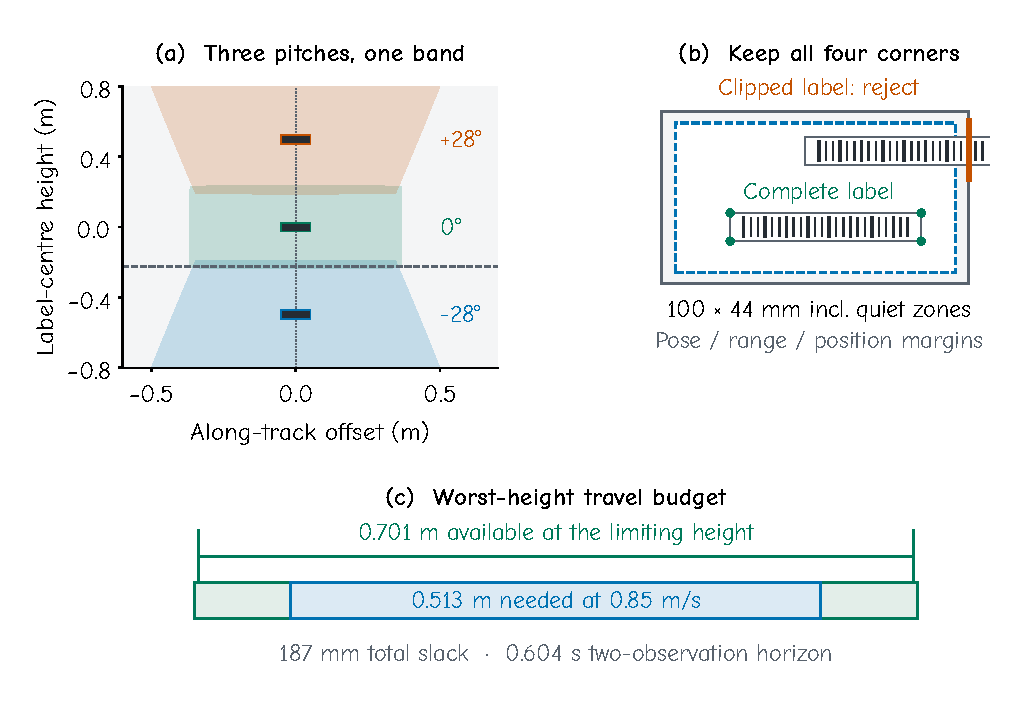
\includegraphics[width=\textwidth]{figures/05_imaging.pdf}
\captionof{figure}{Whole-label admission: (a) three-pitch coverage on the rack face; (b) corner containment schematic; (c) limiting travel budget.}\label{fig:4}\end{minipage}\par\addvspace{2pt}
\subsection{P{\fontsize{9.2}{14}\selectfont ROPULSION} {\fontsize{9.2}{14}\selectfont AND} {\fontsize{9.2}{14}\selectfont SHARED}-{\fontsize{9.2}{14}\selectfont CURRENT} {\fontsize{9.2}{14}\selectfont AUTHORITY}}
MN3508 KV380 manufacturer tests at 22.2 V give P14×4.8 samples of 710 g/64.38 W, 1100 g/117.66 W, 1350 g/166.5 W, 1580 g/217.56 W and 1730 g/255.3 W per motor \cite{r6}. Our 725.4 g-per-rotor hover lies within the first interval. With thrusts expressed in newtons, interpolation gives 265.94 W for four rotors:
\begin{equation}P_h=4\left[P_1+\frac{T_h-T_1}{T_2-T_1}(P_2-P_1)\right],\qquad T_h=mg/4.\end{equation}
Installation power multipliers are 1.10 nominal and 1.25 adverse. Maximum thrust is screened by $(V/22.2)^2$ and a 0.85 derating. The power map and the voltage ceiling are distinct assumptions. Below the first 710 g point, its power is retained as a monotonic upper bound rather than extrapolated to zero. Applying the shared current constraint gives:

\par\addvspace{8pt}\noindent\begin{minipage}{\linewidth}\centering
\captionof{table}{Modelled authority with a 60 W auxiliary load and 30 A limit.}\label{tab:6}
\begin{tabular}{C{0.260\dimexpr\linewidth-32pt\relax}C{0.250\dimexpr\linewidth-32pt\relax}C{0.250\dimexpr\linewidth-32pt\relax}C{0.240\dimexpr\linewidth-32pt\relax}}
\toprule
\textbf{Bus (V)} & \textbf{Collective T/W} & \textbf{Roll/pitch torque (N m)} & \textbf{20\% differential current (A)}\\\midrule
22.2 & 1.541 & 5.629 & 19.67\\
19.8 & 1.407 & 3.697 & 22.06\\
18.0 & 1.298 & 2.008 & 24.26\\
\bottomrule\end{tabular}\end{minipage}\par\addvspace{8pt}
Torque is the single-axis bound at hover collective; simultaneous roll/pitch/yaw demands share that envelope. A 20\% rotor-pair differential supplies 1.207 N m, and steady 12° tilt fits the model at 18 V. The matched rigid-body test below checks combined manoeuvres using the same allocator. The voltage-squared ceiling supplies the engineering estimate pending a loaded low-voltage motor test.

\par\addvspace{2pt}\noindent\begin{minipage}{\linewidth}\centering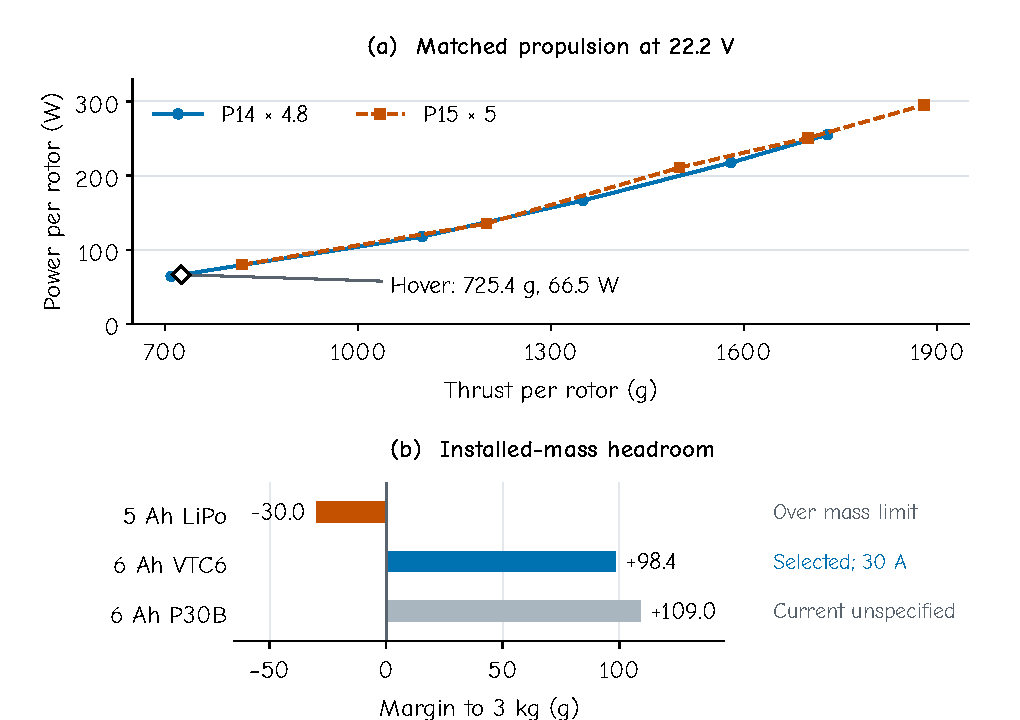
\includegraphics[width=\textwidth]{figures/02_propulsion.pdf}
\captionof{figure}{Manufacturer power samples at 22.2 V \cite{r6} and installed-mass margin to 3 kg. The diamond marks hover interpolation.}\label{fig:5}\end{minipage}\par\addvspace{2pt}
\subsection{M{\fontsize{9.2}{14}\selectfont ISSION} {\fontsize{9.2}{14}\selectfont DURATION} {\fontsize{9.2}{14}\selectfont AND} {\fontsize{9.2}{14}\selectfont ENERGY}}
Five bilateral passes require 400 m scan travel; return and launch approach add 84 m horizontally. Launch and end manoeuvres use observed-free staging volumes beyond the rack ends. Their availability is an installation condition, separate from the specified aisle dimensions. Scan speed is 0.85 m/s, vertical speed is 0.35 m/s and acceleration is 0.6 m/s². Rest-to-rest travel over distance $d$ at speed limit $v$ takes:
\begin{equation}t(d)=\begin{cases}2\sqrt{d/a},&d\le v^2/a,\\ d/v+v/a,&d>v^2/a.\end{cases}\end{equation}
Initialisation allocates 5 s to stationary alignment, 3 s to local-plane acquisition and 2 s to health/admission checks. Five turn events (including the return turn) each receive 0.5 s confirmation and 4 s yaw/reacquisition; ten boundary holds each consume one 0.60 s optical cycle. Discovery runs during the first scan. Unresolved geometry pauses the scan and consumes the remaining dwell allowance.

A failed item adds 7.66 s for processing, braking/resumption, recentering and two 0.5 s settled attempts. Optional lateral approach/return adds 2.61 s, including 0.30 s settling. Thus two, eight and twenty recovered items add 20.53, 82.14 and 205.32 s. Recovery counts are workload scenarios.

\par\addvspace{8pt}\noindent\begin{minipage}{\linewidth}\centering
\captionof{table}{Mission budget with two full local recoveries.}\label{tab:7}
\begin{tabular}{C{0.260\dimexpr\linewidth-32pt\relax}C{0.250\dimexpr\linewidth-32pt\relax}C{0.250\dimexpr\linewidth-32pt\relax}C{0.240\dimexpr\linewidth-32pt\relax}}
\toprule
\textbf{Phase} & \textbf{Time (s)} & \textbf{Nominal (Wh)} & \textbf{Adverse (Wh)}\\\midrule
Takeoff & 2.2 & 0.22 & 0.26\\
Approach & 3.7 & 0.35 & 0.40\\
Scan & 477.7 & 46.23 & 52.20\\
Climb & 20.6 & 2.07 & 2.52\\
Return & 85.3 & 8.26 & 9.33\\
Descend & 18.9 & 1.82 & 2.23\\
Land & 2.2 & 0.21 & 0.25\\
Initialization & 10.0 & 0.97 & 1.09\\
Endpoint observation & 2.5 & 0.24 & 0.27\\
Yaw and reacquisition & 20.0 & 1.93 & 2.18\\
Boundary pairs & 6.0 & 0.58 & 0.65\\
Targeted retries & 15.3 & 1.48 & 1.67\\
Lateral recovery & 5.2 & 0.50 & 0.57\\
\textbf{Total} & \textbf{669.5} & \textbf{64.86} & \textbf{73.63}\\
\bottomrule\end{tabular}\end{minipage}\par\addvspace{8pt}
The phase-power model separates installed hover loss, horizontal tilt/drag and positive climbing work. With installation factor $k$, drag area $C_D A=0.15~\mathrm{m}^2$ and phase duration $t_j$:
\begin{equation}E_j=\frac{\left[kP_h(1+(a/g)^2)^{3/4}+P_{aux}+\tfrac12\rho C_D A v^3\right]t_j+mg\max(0,\Delta z_j)/\eta_z}{3600}.\end{equation}
Vertical phases omit horizontal terms and use $\eta_z=0.60$; the adverse vertical multiplier is 1.10. Auxiliary load is 55/60 W nominal/adverse, with no descent energy credit. Applying the small tilt increment across a horizontal segment is our modelling approximation; loaded tests identify installation and rack-interaction losses.

VTC6 cell data specify 3.6 V nominal and rate-dependent loaded discharge \cite{r38}. The 12-cell nameplate is 129.6 Wh. The original 19.8 V cutoff is rejected: the digitised typical 10 A/cell curve supplies only 87.66 Wh before connection losses, below the 92.04 Wh delivered-energy requirement. The revised candidate uses an 18.0 V loaded cutoff, retaining the same pack and mass.

Loaded voltage, current and delivered energy are solved together:
\begin{equation}V=6v_c(q,I/2)-IR_b,\quad P=VI,\quad \dot q=I/(2\times3600),\quad E_{bus}=\int VI\,dt/3600.\end{equation}
Recorded axis calibration digitises the 23 °C, 10/15 A curves. Voltage is interpolated between them; below 10 A/cell, the 10 A curve bounds rate loss. Cell drop is already included. Assembly resistance adds $IR_b$ drop and $I^2R_b$ loss. Screening uses 10 mΩ, a −40 mV/cell shift and 3000/3120 capacity-axis scale: explicit sensitivities rather than a guaranteed minimum-cell curve.

After the adverse mission, remaining deliverable energy is integrated at the largest phase-average load, 440.38 W. Reserve is $E_{remaining}/(E_{mission}+E_{remaining})$. The resulting delivered energy is about 100.4 Wh for the two-recovery load history. The 72-case sweep varies cutoff, connection resistance, capacity and recovery count; high-load-first/last ordering changes tested reserve by less than 0.04 percentage points.

\par\addvspace{2pt}\noindent\begin{minipage}{\linewidth}\centering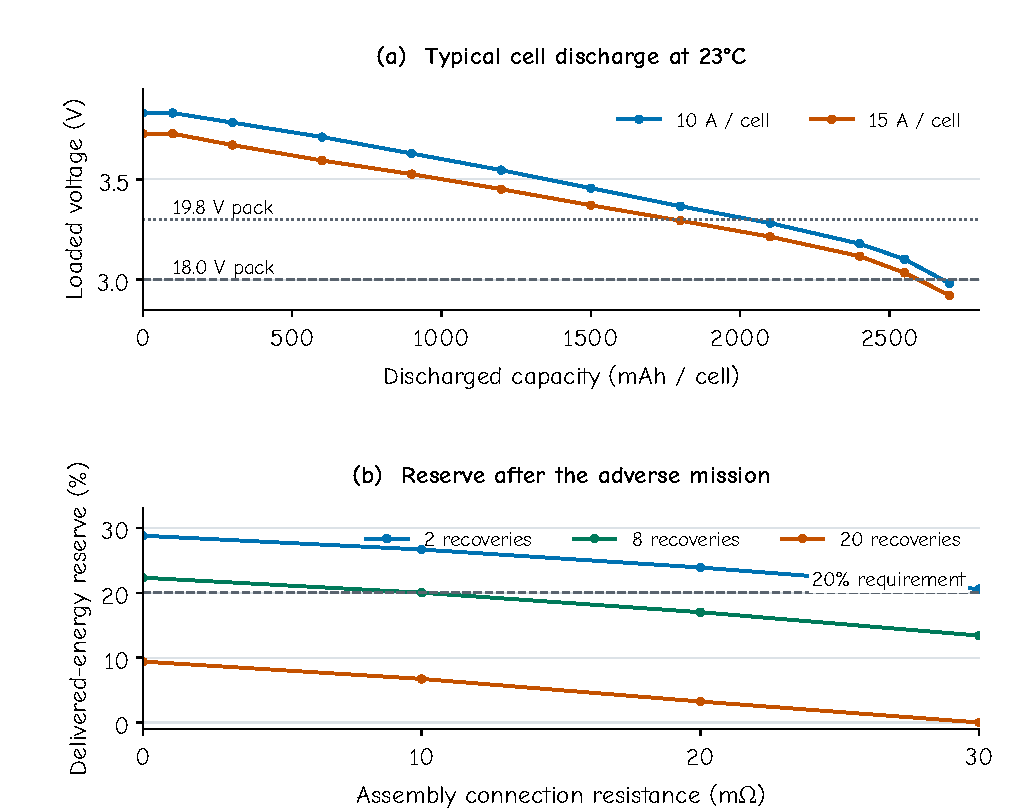
\includegraphics[width=\textwidth]{figures/07_energy.pdf}
\captionof{figure}{Loaded-pack evidence and recovery reserve at 18 V. Curves use manufacturer cell data with stated capacity and voltage sensitivities.}\label{fig:6}\end{minipage}\par\addvspace{2pt}
\par\addvspace{8pt}\noindent\begin{minipage}{\linewidth}\centering
\captionof{table}{Recovery workload and delivered-energy reserve; 23 °C model.}\label{tab:8}
\begin{tabular}{C{0.200\dimexpr\linewidth-40pt\relax}C{0.200\dimexpr\linewidth-40pt\relax}C{0.200\dimexpr\linewidth-40pt\relax}C{0.200\dimexpr\linewidth-40pt\relax}C{0.200\dimexpr\linewidth-40pt\relax}}
\toprule
\textbf{Recoveries} & \textbf{Duration (s)} & \textbf{Mission (Wh)} & \textbf{Reserve, 10 mΩ} & \textbf{Reserve, 20 mΩ}\\\midrule
2 & 669.5 & 73.63 & 26.65\% & 23.89\%\\
8 & 731.1 & 80.35 & 20.00\% & 17.00\%\\
20 & 854.3 & 93.78 & 6.72\% & 3.23\%\\
\bottomrule\end{tabular}\end{minipage}\par\addvspace{8pt}
The selected screening case admits two recoveries with useful margin; eight reaches the reserve boundary. At 20 mΩ, eight leave about 17.0\% reserve. With 90\% capacity-axis scale and 20 mΩ, even two leave about 18.7\%. These cases are rejected by the 20\% rule. Recovery count is not a measured failure probability: the planner updates unfinished work, return energy and remaining dwell after every discovery. A persistent unreadable item remains an exception, never a completed inventory record. Pack resistance/capacity, individual-cell undervoltage protection, temperature and loaded motor maps determine physical release.

\section{E{\fontsize{11.2}{14}\selectfont XPERIMENTAL} E{\fontsize{11.2}{14}\selectfont VALUATION}}
\subsection{I{\fontsize{9.2}{14}\selectfont MPLEMENTATION} {\fontsize{9.2}{14}\selectfont AND} {\fontsize{9.2}{14}\selectfont EVALUATION} {\fontsize{9.2}{14}\selectfont CONDITIONS}}
We built a MuJoCo reference environment for flight tracking, continuous multilevel scanning and image-based inventory \cite{r27}. We use a Skydio X2 mesh from MuJoCo Menagerie, Poly Haven carton/shelf assets, and project geometry for primary rack supports and pallets \cite{r30,r31,r32}. The plant integrates free-body dynamics, four thrust sites, actuator lag, bounded control, contacts and bilateral rendered cameras. Table 9 identifies the configuration used for the recorded experiments alongside the proposed hardware.

\par\addvspace{8pt}\noindent\begin{minipage}{\linewidth}\centering
\captionof{table}{Design and experimental configurations.}\label{tab:9}
\begin{tabular}{C{0.290\dimexpr\linewidth-24pt\relax}C{0.290\dimexpr\linewidth-24pt\relax}C{0.420\dimexpr\linewidth-24pt\relax}}
\toprule
\textbf{Parameter} & \textbf{Proposed aircraft} & \textbf{Reference experiment}\\\midrule
Installed mass & 2901.6 g allocation & 2.65 kg rigid body\\
Envelope & 1.00 m diameter; 0.50 m height & 0.80 m diameter; 0.29 m height\\
Battery & 6S2P 6 Ah; loaded cutoff 18.0 V & 4S 6 Ah model; 88.8 Wh\\
Propulsion & Matched table + installation factors & 330 W induced-power reference\\
Optics & 4096×3000; 12 mm; pitch sweep & 4096×2160; 45° horizontal; fixed\\
Scan speed & 0.85 m/s optical limit & 1.1 m/s prescribed route\\
Navigation & LiDAR/IMU/image estimator & Delayed/noisy position/velocity; ideal attitude\\
\bottomrule\end{tabular}\end{minipage}\par\addvspace{8pt}
The reference run isolates tracking and decoding with a prescribed route and state proxies. The 136 s film replays its 501.02 s flight in 72 s (6.96×), using saved-pose external, side and forward views at 30 fps. The local revision updates the design-analysis card; the linked upload presents the earlier reference film.

\subsection{C{\fontsize{9.2}{14}\selectfont ONTROLLER} {\fontsize{9.2}{14}\selectfont SELECTION} {\fontsize{9.2}{14}\selectfont AND} {\fontsize{9.2}{14}\selectfont COMPLETE}-{\fontsize{9.2}{14}\selectfont ROUTE} {\fontsize{9.2}{14}\selectfont TRACKING}}
Physics runs at 200 Hz and control at 50 Hz, with 40 ms motor response and four 13 N actuator limits. A bounded acceleration residual augments position/velocity feedback, following residual reinforcement learning \cite{r28}. PPO uses two 128-unit hidden layers \cite{r29}. Three seeds each completed one million steps of local sinusoidal tracking with randomised mass, motor response, authority and wind. The mission planner supplies the full serpentine reference.

We compare validation-best and final checkpoints from all three seeds plus the baseline on two selection routes: seeds 701/702 and 0/1 N wind. We then test the selected controller separately on seed 703 with 0.5 N wind.

\par\addvspace{8pt}\noindent\begin{minipage}{\linewidth}\centering
\captionof{table}{Mean position RMSE across two selection conditions.}\label{tab:10}
\begin{tabular}{C{0.290\dimexpr\linewidth-24pt\relax}C{0.290\dimexpr\linewidth-24pt\relax}C{0.420\dimexpr\linewidth-24pt\relax}}
\toprule
\textbf{Controller / checkpoint} & \textbf{Mean RMSE (m)} & \textbf{Selection outcome}\\\midrule
baseline & 0.1056 & Baseline\\
seed0 best & 0.1110 & Comparison\\
seed0 final & 0.1082 & Comparison\\
seed1 best & 0.1280 & Comparison\\
seed1 final & 0.1784 & Comparison\\
\textbf{seed2 best} & \textbf{0.0977} & \textbf{Selected}\\
seed2 final & 0.1137 & Comparison\\
\bottomrule\end{tabular}\end{minipage}\par\addvspace{8pt}
\par\addvspace{8pt}\noindent\begin{minipage}{\linewidth}\centering
\captionof{table}{Separate complete-route comparison; one route per controller.}\label{tab:11}
\begin{tabular}{C{0.190\dimexpr\linewidth-32pt\relax}C{0.190\dimexpr\linewidth-32pt\relax}C{0.190\dimexpr\linewidth-32pt\relax}C{0.430\dimexpr\linewidth-32pt\relax}}
\toprule
\textbf{Measure} & \textbf{Baseline} & \textbf{Residual} & \textbf{Interpretation}\\\midrule
RMSE (m) & 0.1148 & 0.1038 & 9.6\% reduction\\
Position p95 (m) & 0.1364 & 0.1233 & Within-route percentile\\
Duration (s) & 501.02 & 501.02 & Same prescribed route\\
Collision & None & None & MuJoCo contact log\\
\bottomrule\end{tabular}\end{minipage}\par\addvspace{8pt}
Seed-2 best achieves the lowest selection RMSE, 0.0977 m against the baseline's 0.1056 m. Full-route RMSE falls by 9.6\%, from 0.1148 to 0.1038 m, over 501.02 s with no contact. Figure~\ref{fig:7} shows the spread across checkpoints and the effect of validation-based selection. The full-route score is 0.0038 m above the 0.10 m objective.

\par\addvspace{2pt}\noindent\begin{minipage}{\linewidth}\centering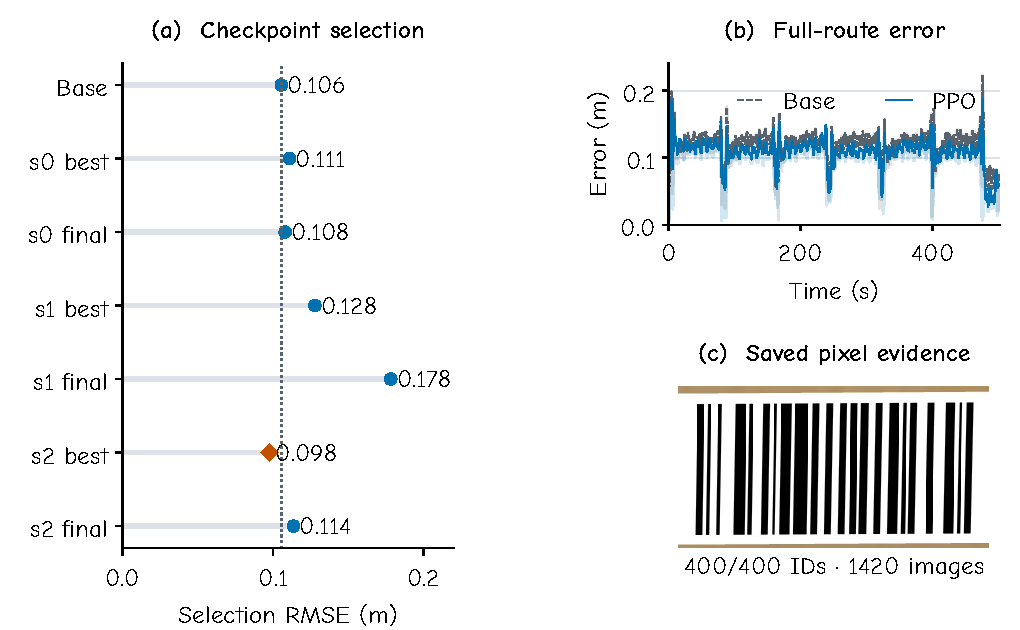
\includegraphics[width=\textwidth]{figures/08_experiment.pdf}
\captionof{figure}{Experimental evidence: all candidate scores, full-route error envelopes (1 s min/max) and a native barcode crop.}\label{fig:7}\end{minipage}\par\addvspace{2pt}
The recorded trajectory alternates forward/reverse 80 m passes and climbs at the current endpoint. Scan/climb/return boundary clearance reaches a minimum of 0.500 m. The full-run 0.068 m minimum includes launch-surface proximity. Boundary distance and MuJoCo scene-contact detection describe different geometries; online operation queries mapped obstacles using the swept envelope.

\subsection{B{\fontsize{9.2}{14}\selectfont ARCODE} {\fontsize{9.2}{14}\selectfont DECODING} {\fontsize{9.2}{14}\selectfont AND} {\fontsize{9.2}{14}\selectfont EVIDENCE}}
We swept label size, exposure, speed and brightness over 720 images, obtaining 439 correct decodes and no incorrect payloads across those mixed conditions. This study motivates joint sampling/exposure selection. Processing 1420 rendered side images from the scene produced 400 correct IDs and two singleton misreads. We re-decoded saved crops using original, resized and Otsu-thresholded pixels; consistency filtering rejected both extra candidates, leaving 400 correct IDs with no omissions. Ground-truth inventory enters only the final scorer.

Crop filtering tests within-image processing consistency. Temporal confirmation uses separate acquisitions and Section 3.5 recovery; matched optical checks test paired viewpoints.

\subsection{M{\fontsize{9.2}{14}\selectfont ATCHED} {\fontsize{9.2}{14}\selectfont DESIGN} {\fontsize{9.2}{14}\selectfont CHECKS}}
The matched design plant uses 2.9016 kg, the 600 mm rotor diagonal, full component-derived inertia, 1.00×0.50 m collision envelope and y=±0.40 m camera centres. Camera bodies and lenses follow manufacturer dimensions. Kinematic head transforms reproduce −28/0/+28° views; servo dynamics and loaded settling are not simulated. The matched warehouse retains the 80×2.5×8 m aisle, five levels, both racks and original 100×44 mm labels. Added ceiling/end boundaries test geometry without changing historical records.

Three 32 s manoeuvre checks use delayed/noisy position/velocity, exact attitude, physical angular dynamics and 40 ms lag. They reach 25.48 A peak current and 5.65° tilt, with 0.0787 m maximum error. Braking to <0.05 m/s takes 1.20 s over 0.527–0.531 m; yaw torque uses the reference coefficient.

The matched plant also executes the complete 669.5 s known-route schedule in the warehouse, including five turns and two declared recovery injections. RMSE is 0.0138 m, maximum error 0.101 m and peak model current 25.84 A. Nominal wall/ceiling clearance remains at least 0.487 m. State proxies and scheduled recoveries isolate flight execution. Online estimation and in-flight decoding are separate integration tasks.

Fourteen native 4096×3000 warehouse exposure pairs test both sides, three height levels and all pitch commands. Both images decode the unchanged 100 mm label in every pair. Static snapshots exclude servo motion and distortion. Fifty-six located-crop perturbations (0.75-pixel blur, brightness 1/0.4, noise 3 DN) retain the expected code without extra candidates. Three hundred numerical rotation cases verify projected derivatives and finite corners against the analytical bounds. Views, crops, traces and source hashes are retained.

\section{D{\fontsize{11.2}{14}\selectfont ISCUSSION} {\fontsize{11.2}{14}\selectfont AND} C{\fontsize{11.2}{14}\selectfont ONCLUSION}}
AWISU couples platform, control and GPS-free navigation through optical, dynamic and energy budgets. Complete-label geometry supports 0.85 m/s acquisition of the reference 100 mm short codes within stated pose errors. Module density identifies when revised optics or closer views are needed.

The 18.0 V cutoff trades collective authority, reduced to 1.30, for mission energy. Matched known-route execution fits the 30 A model limit, and native image pairs decode the retained labels. Physical release requires loaded pack/motor characterisation and integrated unknown-layout estimation and coverage.

\renewcommand{\refname}{R{\fontsize{11.2}{14}\selectfont EFERENCES}}\begin{thebibliography}{99}\interlinepenalty=10000\renewcommand{\makelabel}[1]{\hfill#1}\setlength{\itemsep}{1pt}\setlength{\parskip}{0pt}
\bibitem{r3} \href{https://www.corvus-robotics.com/corvus-one}{Corvus Robotics, Corvus One}.
\bibitem{r4} \href{https://www.verity.net/}{Verity, Warehouse Intelligence}.
\bibitem{r5} \href{https://docs.holybro.com/drone-development-kit/px4-development-kit-x500v2}{Holybro, X500 v2 development kit}.
\bibitem{r6} \href{https://store.tmotor.com/product/mn3508-motor-navigator-type.html}{T-MOTOR, MN3508 Navigator motor}.
\bibitem{r7} \href{https://store.tmotor.com/product/air-40a-6s-esc.html}{T-MOTOR, AIR 40A 2-6S ESC}.
\bibitem{r8} \href{https://store.tmotor.com/product/polish-carbon-fiber-14x4_8-prop.html}{T-MOTOR, P14x4.8 carbon propeller}.
\bibitem{r9} \href{https://www.genstattu.com/content/instock/rc_product_brochure.pdf}{Gens ace / Tattu, RC product brochure}.
\bibitem{r10} \href{https://holybro.com/products/pixhawk-6c}{Holybro, Pixhawk 6C}.
\bibitem{r11} \href{https://holybro.com/collections/power-modules-pdbs/products/pm02-v3-12s-power-module}{Holybro, PM02 V3 analog power module}.
\bibitem{r12} \href{https://www.livoxtech.com/mid-360/specs}{Livox, MID-360 specifications}.
\bibitem{r13} \href{https://docs.luxonis.com/hardware/products/OAK-D%20Lite}{Luxonis, OAK-D Lite}.
\bibitem{r14} \href{https://developer.nvidia.com/embedded/jetson-modules}{NVIDIA, Jetson module lineup}.
\bibitem{r15} \href{https://www.hiwonder.com/products/mini-carrier}{Hiwonder, Jetson Mini carrier}.
\bibitem{r16} \href{https://softwareservices.flir.com/BFS-U3-51S5/latest/Model/spec.html}{Teledyne FLIR, BFS-U3-51S5 specifications}.
\bibitem{r17} \href{https://kowa-fa-sea.com.sg/industrial-lens/jc5mc-series/}{Kowa, JC5MC lens series: LM8JC5MC and LM12JC5MC}.
\bibitem{r18} \href{https://torqpro.com/product/mg90s-analog/}{TowerPro, MG90S Analog pitch servo}.
\bibitem{r19} \href{https://arxiv.org/abs/2107.06829}{Wei Xu, Yixi Cai, Dongjiao He, Jiarong Lin, and Fu Zhang. FAST-LIO2: Fast Direct LiDAR-inertial Odometry. arXiv:2107.06829, 2021}.
\bibitem{r20} \href{https://arxiv.org/abs/2007.11898}{Carlos Campos, Richard Elvira, Juan J. Gómez Rodríguez, José M. M. Montiel, and Juan D. Tardós. ORB-SLAM3: An Accurate Open-Source Library for Visual, Visual-Inertial and Multi-Map SLAM. arXiv:2007.11898, 2021}.
\bibitem{r21} \href{https://arxiv.org/abs/2408.14035}{Chunran Zheng et al. FAST-LIVO2: Fast, Direct LiDAR-Inertial-Visual Odometry. arXiv:2408.14035, 2024}.
\bibitem{r22} \href{https://arxiv.org/abs/2001.04420}{Jesus Tordesillas, Brett T. Lopez, Michael Everett, and Jonathan P. How. FASTER: Fast and Safe Trajectory Planner for Navigation in Unknown Environments. arXiv:2001.04420, 2021}.
\bibitem{r23} \href{https://docs.px4.io/main/en/ros/external_position_estimation}{PX4, external position estimation}.
\bibitem{r24} \href{https://docs.px4.io/main/en/flight_modes/offboard}{PX4, Offboard mode}.
\bibitem{r25} \href{https://doi.org/10.1007/s10514-012-9321-0}{Armin Hornung, Kai M. Wurm, Maren Bennewitz, Cyrill Stachniss, and Wolfram Burgard. OctoMap: An Efficient Probabilistic 3D Mapping Framework Based on Octrees. Autonomous Robots, 34:189–206, 2013}.
\bibitem{r26} \href{https://github.com/zxing-cpp/zxing-cpp}{zxing-cpp reference implementation}.
\bibitem{r27} \href{https://mujoco.readthedocs.io/en/stable/overview.html}{MuJoCo documentation}.
\bibitem{r28} \href{https://arxiv.org/abs/1812.03201}{Tobias Johannink et al. Residual Reinforcement Learning for Robot Control. arXiv:1812.03201, 2018}.
\bibitem{r29} \href{https://arxiv.org/abs/1707.06347}{John Schulman, Filip Wolski, Prafulla Dhariwal, Alec Radford, and Oleg Klimov. Proximal Policy Optimization Algorithms. arXiv:1707.06347, 2017}.
\bibitem{r30} \href{https://github.com/google-deepmind/mujoco_menagerie/tree/main/skydio_x2}{MuJoCo Menagerie, Skydio X2}.
\bibitem{r31} \href{https://polyhaven.com/a/cardboard_box_01}{Poly Haven, Cardboard Box 01}.
\bibitem{r32} \href{https://polyhaven.com/a/steel_frame_shelves_03}{Poly Haven, Steel Frame Shelves 03}.
\bibitem{r33} \href{https://www.pololu.com/product/4095}{Pololu, D36V50F12 regulator}.
\bibitem{r34} \href{https://lumileds.com/products/high-power-leds/luxeon-rebel/}{Lumileds LUXEON Rebel emitters; Texas Instruments TPS92512 LED driver}.
\bibitem{r35} \href{https://softwareservices.flir.com/BFS-U3-122S6/latest/Model/spec.html}{Teledyne FLIR, BFS-U3-122S6 specifications}.
\bibitem{r36} \href{https://www.opto-e.com/en/products/en-12rt-series/RT-V1228-MPY2}{Opto Engineering RT-V1228-MPY2 catalogue}.
\bibitem{r37} \href{https://geprc.com/product/geprc-vtc6-18650-6s2p-6000mah-batteries/}{GEPRC VTC6 6S2P6000 pack}.
\bibitem{r38} \href{https://www.murata.com/-/media/webrenewal/products/batteries/cylindrical/datasheet/us18650vtc6-product-datasheet.ashx}{Murata VTC6 cell datasheet}.
\bibitem{r39} \href{https://flywoo.net/products/flywoo-explorer-molicell-p30b-18650-6s2p-6000mah-lionpack-battery}{Flywoo P30B 6S2P6000 pack}.
\bibitem{r40} \href{https://www.math.ucsd.edu/~mleok/pdf/LeLeMc2010_quadrotor.pdf}{Taeyoung Lee, Melvin Leok, and N. Harris McClamroch. Geometric Tracking Control of a Quadrotor UAV on SE(3). IEEE Conference on Decision and Control, 2010}.
\bibitem{r41} \href{https://arxiv.org/abs/1611.09240}{Mina Kamel, Michael Burri, and Roland Siegwart. Linear vs Nonlinear MPC for Trajectory Tracking Applied to Rotary Wing Micro Aerial Vehicles. arXiv:1611.09240, 2017}.
\bibitem{r42} \href{https://docs.px4.io/main/en/flight_stack/controller_diagrams}{PX4 controller diagrams}.
\bibitem{r43} \href{https://github.com/hku-mars/FAST-LIVO2}{HKU MARS, FAST-LIVO2 official implementation}.
\bibitem{r44} \href{https://www.lumenier.com/products/lumenier-nav-6000mah-6s-21700-amprius-lithium-ion-battery-xt60}{Lumenier NAV Amprius6S6000 pack}.
\bibitem{r45} \href{https://liberzon.csl.illinois.edu/teaching/kalman_paper.pdf}{R. E. Kalman, Contributions to the Theory of Optimal Control, Bol. Soc. Mat. Mex. 5, 102–119, 1960}.
\bibitem{r46} \href{https://arxiv.org/abs/2609.00065}{Kassis, Agarwal, He, Patel and Brueckner, Scientific Agent Skills: A Library of Procedural Knowledge for Research Agents, 2026}.
\end{thebibliography}
\end{document}
